\documentclass[1p]{elsarticle_modified}
%\bibliographystyle{elsarticle-num}

%\usepackage[colorlinks]{hyperref}
%\usepackage{abbrmath_seonhwa} %\Abb, \Ascr, \Acal ,\Abf, \Afrak
\usepackage{amsfonts}
\usepackage{amssymb}
\usepackage{amsmath}
\usepackage{amsthm}
\usepackage{scalefnt}
\usepackage{amsbsy}
\usepackage{kotex}
\usepackage{caption}
\usepackage{subfig}
\usepackage{color}
\usepackage{graphicx}
\usepackage{xcolor} %% white, black, red, green, blue, cyan, magenta, yellow
\usepackage{float}
\usepackage{setspace}
\usepackage{hyperref}

\usepackage{tikz}
\usetikzlibrary{arrows}

\usepackage{multirow}
\usepackage{array} % fixed length table
\usepackage{hhline}

%%%%%%%%%%%%%%%%%%%%%
\makeatletter
\renewcommand*\env@matrix[1][\arraystretch]{%
	\edef\arraystretch{#1}%
	\hskip -\arraycolsep
	\let\@ifnextchar\new@ifnextchar
	\array{*\c@MaxMatrixCols c}}
\makeatother %https://tex.stackexchange.com/questions/14071/how-can-i-increase-the-line-spacing-in-a-matrix
%%%%%%%%%%%%%%%

\usepackage[normalem]{ulem}

\newcommand{\msout}[1]{\ifmmode\text{\sout{\ensuremath{#1}}}\else\sout{#1}\fi}
%SOURCE: \msout is \stkout macro in https://tex.stackexchange.com/questions/20609/strikeout-in-math-mode

\newcommand{\cancel}[1]{
	\ifmmode
	{\color{red}\msout{#1}}
	\else
	{\color{red}\sout{#1}}
	\fi
}

\newcommand{\add}[1]{
	{\color{blue}\uwave{#1}}
}

\newcommand{\replace}[2]{
	\ifmmode
	{\color{red}\msout{#1}}{\color{blue}\uwave{#2}}
	\else
	{\color{red}\sout{#1}}{\color{blue}\uwave{#2}}
	\fi
}

\newcommand{\Sol}{\mathcal{S}} %segment
\newcommand{\D}{D} %diagram
\newcommand{\A}{\mathcal{A}} %arc


%%%%%%%%%%%%%%%%%%%%%%%%%%%%%5 test

\def\sl{\operatorname{\textup{SL}}(2,\Cbb)}
\def\psl{\operatorname{\textup{PSL}}(2,\Cbb)}
\def\quan{\mkern 1mu \triangleright \mkern 1mu}

\theoremstyle{definition}
\newtheorem{thm}{Theorem}[section]
\newtheorem{prop}[thm]{Proposition}
\newtheorem{lem}[thm]{Lemma}
\newtheorem{ques}[thm]{Question}
\newtheorem{cor}[thm]{Corollary}
\newtheorem{defn}[thm]{Definition}
\newtheorem{exam}[thm]{Example}
\newtheorem{rmk}[thm]{Remark}
\newtheorem{alg}[thm]{Algorithm}

\newcommand{\I}{\sqrt{-1}}
\begin{document}

%\begin{frontmatter}
%
%\title{Boundary parabolic representations of knots up to 8 crossings}
%
%%% Group authors per affiliation:
%\author{Yunhi Cho} 
%\address{Department of Mathematics, University of Seoul, Seoul, Korea}
%\ead{yhcho@uos.ac.kr}
%
%
%\author{Seonhwa Kim} %\fnref{s_kim}}
%\address{Center for Geometry and Physics, Institute for Basic Science, Pohang, 37673, Korea}
%\ead{ryeona17@ibs.re.kr}
%
%\author{Hyuk Kim}
%\address{Department of Mathematical Sciences, Seoul National University, Seoul 08826, Korea}
%\ead{hyukkim@snu.ac.kr}
%
%\author{Seokbeom Yoon}
%\address{Department of Mathematical Sciences, Seoul National University, Seoul, 08826,  Korea}
%\ead{sbyoon15@snu.ac.kr}
%
%\begin{abstract}
%We find all boundary parabolic representation of knots up to 8 crossings.
%
%\end{abstract}
%\begin{keyword}
%    \MSC[2010] 57M25 
%\end{keyword}
%
%\end{frontmatter}

%\linenumbers
%\tableofcontents
%
\newcommand\colored[1]{\textcolor{white}{\rule[-0.35ex]{0.8em}{1.4ex}}\kern-0.8em\color{red} #1}%
%\newcommand\colored[1]{\textcolor{white}{ #1}\kern-2.17ex	\textcolor{white}{ #1}\kern-1.81ex	\textcolor{white}{ #1}\kern-2.15ex\color{red}#1	}

{\Large $\underline{12n_{0195}~(K12n_{0195})}$}

\setlength{\tabcolsep}{10pt}
\renewcommand{\arraystretch}{1.6}
\vspace{1cm}\begin{tabular}{m{100pt}>{\centering\arraybackslash}m{274pt}}
\multirow{5}{120pt}{
	\centering
	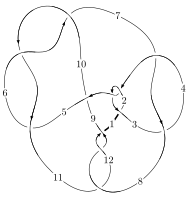
\includegraphics[width=112pt]{../../../GIT/diagram.site/Diagrams/png/2284_12n_0195.png}\\
\ \ \ A knot diagram\footnotemark}&
\allowdisplaybreaks
\textbf{Linearized knot diagam} \\
\cline{2-2}
 &
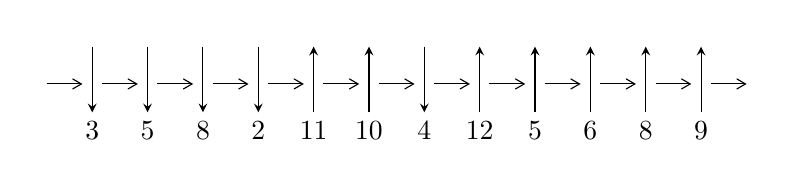
\begin{tikzpicture}[x=20pt, y=17pt]
	% nodes
	\node (C0) at (0, 0) {};
	\node (C1) at (1, 0) {};
	\node (C1U) at (1, +1) {};
	\node (C1D) at (1, -1) {3};

	\node (C2) at (2, 0) {};
	\node (C2U) at (2, +1) {};
	\node (C2D) at (2, -1) {5};

	\node (C3) at (3, 0) {};
	\node (C3U) at (3, +1) {};
	\node (C3D) at (3, -1) {8};

	\node (C4) at (4, 0) {};
	\node (C4U) at (4, +1) {};
	\node (C4D) at (4, -1) {2};

	\node (C5) at (5, 0) {};
	\node (C5U) at (5, +1) {};
	\node (C5D) at (5, -1) {11};

	\node (C6) at (6, 0) {};
	\node (C6U) at (6, +1) {};
	\node (C6D) at (6, -1) {10};

	\node (C7) at (7, 0) {};
	\node (C7U) at (7, +1) {};
	\node (C7D) at (7, -1) {4};

	\node (C8) at (8, 0) {};
	\node (C8U) at (8, +1) {};
	\node (C8D) at (8, -1) {12};

	\node (C9) at (9, 0) {};
	\node (C9U) at (9, +1) {};
	\node (C9D) at (9, -1) {5};

	\node (C10) at (10, 0) {};
	\node (C10U) at (10, +1) {};
	\node (C10D) at (10, -1) {6};

	\node (C11) at (11, 0) {};
	\node (C11U) at (11, +1) {};
	\node (C11D) at (11, -1) {8};

	\node (C12) at (12, 0) {};
	\node (C12U) at (12, +1) {};
	\node (C12D) at (12, -1) {9};
	\node (C13) at (13, 0) {};

	% arrows
	\draw[->,>={angle 60}]
	(C0) edge (C1) (C1) edge (C2) (C2) edge (C3) (C3) edge (C4) (C4) edge (C5) (C5) edge (C6) (C6) edge (C7) (C7) edge (C8) (C8) edge (C9) (C9) edge (C10) (C10) edge (C11) (C11) edge (C12) (C12) edge (C13) ;	\draw[->,>=stealth]
	(C1U) edge (C1D) (C2U) edge (C2D) (C3U) edge (C3D) (C4U) edge (C4D) (C5D) edge (C5U) (C6D) edge (C6U) (C7U) edge (C7D) (C8D) edge (C8U) (C9D) edge (C9U) (C10D) edge (C10U) (C11D) edge (C11U) (C12D) edge (C12U) ;
	\end{tikzpicture} \\
\hhline{~~} \\& 
\textbf{Solving Sequence} \\ \cline{2-2} 
 &
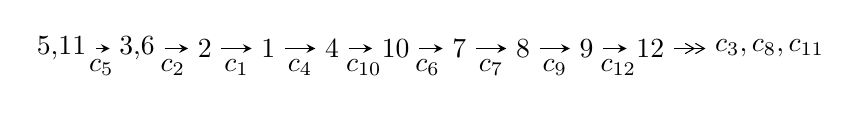
\begin{tikzpicture}[x=23pt, y=7pt]
	% node
	\node (A0) at (-1/8, 0) {5,11};
	\node (A1) at (17/16, 0) {3,6};
	\node (A2) at (17/8, 0) {2};
	\node (A3) at (25/8, 0) {1};
	\node (A4) at (33/8, 0) {4};
	\node (A5) at (41/8, 0) {10};
	\node (A6) at (49/8, 0) {7};
	\node (A7) at (57/8, 0) {8};
	\node (A8) at (65/8, 0) {9};
	\node (A9) at (73/8, 0) {12};
	\node (C1) at (1/2, -1) {$c_{5}$};
	\node (C2) at (13/8, -1) {$c_{2}$};
	\node (C3) at (21/8, -1) {$c_{1}$};
	\node (C4) at (29/8, -1) {$c_{4}$};
	\node (C5) at (37/8, -1) {$c_{10}$};
	\node (C6) at (45/8, -1) {$c_{6}$};
	\node (C7) at (53/8, -1) {$c_{7}$};
	\node (C8) at (61/8, -1) {$c_{9}$};
	\node (C9) at (69/8, -1) {$c_{12}$};
	\node (A10) at (11, 0) {$c_{3},c_{8},c_{11}$};

	% edge
	\draw[->,>=stealth]	
	(A0) edge (A1) (A1) edge (A2) (A2) edge (A3) (A3) edge (A4) (A4) edge (A5) (A5) edge (A6) (A6) edge (A7) (A7) edge (A8) (A8) edge (A9) ;
	\draw[->>,>={angle 60}]	
	(A9) edge (A10);
\end{tikzpicture} \\ 

\end{tabular} \\

\footnotetext{
The image of knot diagram is generated by the software ``\textbf{Draw programme}" developed by Andrew Bartholomew(\url{http://www.layer8.co.uk/maths/draw/index.htm\#Running-draw}), where we modified some parts for our purpose(\url{https://github.com/CATsTAILs/LinksPainter}).
}\phantom \\ \newline 
\centering \textbf{Ideals for irreducible components\footnotemark of $X_{\text{par}}$} 
 
\begin{align*}
I^u_{1}&=\langle 
-1.62072\times10^{18} u^{23}+1.95726\times10^{19} u^{22}+\cdots+1.72477\times10^{21} b+8.62668\times10^{20},\\
\phantom{I^u_{1}}&\phantom{= \langle  }-2.65800\times10^{20} u^{23}+1.49704\times10^{20} u^{22}+\cdots+1.03486\times10^{22} a-3.34302\times10^{22},\;u^{24}-2 u^{23}+\cdots-8 u-8\rangle \\
I^u_{2}&=\langle 
b+1,\;2 u^5-4 u^4+7 u^3-8 u^2+3 a+6 u-5,\;u^6- u^5+3 u^4-2 u^3+2 u^2- u-1\rangle \\
I^u_{3}&=\langle 
4 a^2 u-6 a^2-8 a u+17 b+12 a+2 u-20,\;4 a^3+6 a^2 u-8 a^2-2 a u- u-6,\;u^2+2\rangle \\
\\
I^v_{1}&=\langle 
a,\;- v^2+b+3 v+1,\;v^3-2 v^2-3 v-1\rangle \\
\end{align*}
\raggedright * 4 irreducible components of $\dim_{\mathbb{C}}=0$, with total 39 representations.\\
\footnotetext{All coefficients of polynomials are rational numbers. But the coefficients are sometimes approximated in decimal forms when there is not enough margin.}
\newpage
\renewcommand{\arraystretch}{1}
\centering \section*{I. $I^u_{1}= \langle -1.62\times10^{18} u^{23}+1.96\times10^{19} u^{22}+\cdots+1.72\times10^{21} b+8.63\times10^{20},\;-2.66\times10^{20} u^{23}+1.50\times10^{20} u^{22}+\cdots+1.03\times10^{22} a-3.34\times10^{22},\;u^{24}-2 u^{23}+\cdots-8 u-8 \rangle$}
\flushleft \textbf{(i) Arc colorings}\\
\begin{tabular}{m{7pt} m{180pt} m{7pt} m{180pt} }
\flushright $a_{5}=$&$\begin{pmatrix}1\\0\end{pmatrix}$ \\
\flushright $a_{11}=$&$\begin{pmatrix}0\\u\end{pmatrix}$ \\
\flushright $a_{3}=$&$\begin{pmatrix}0.0256846 u^{23}-0.0144661 u^{22}+\cdots-1.52339 u+3.23040\\0.000939669 u^{23}-0.0113479 u^{22}+\cdots+0.985369 u-0.500163\end{pmatrix}$ \\
\flushright $a_{6}=$&$\begin{pmatrix}1\\- u^2\end{pmatrix}$ \\
\flushright $a_{2}=$&$\begin{pmatrix}0.0266242 u^{23}-0.0258140 u^{22}+\cdots-0.538021 u+2.73023\\0.000939669 u^{23}-0.0113479 u^{22}+\cdots+0.985369 u-0.500163\end{pmatrix}$ \\
\flushright $a_{1}=$&$\begin{pmatrix}0.0583259 u^{23}-0.126312 u^{22}+\cdots+3.65005 u+0.821695\\-0.0138991 u^{23}+0.0340693 u^{22}+\cdots+0.0978404 u-0.00653011\end{pmatrix}$ \\
\flushright $a_{4}=$&$\begin{pmatrix}0.00790799 u^{23}+0.00662412 u^{22}+\cdots-2.90944 u+2.73115\\-0.00229500 u^{23}-0.00348046 u^{22}+\cdots+1.12451 u-0.423114\end{pmatrix}$ \\
\flushright $a_{10}=$&$\begin{pmatrix}- u\\u^3+u\end{pmatrix}$ \\
\flushright $a_{7}=$&$\begin{pmatrix}u^2+1\\- u^4-2 u^2\end{pmatrix}$ \\
\flushright $a_{8}=$&$\begin{pmatrix}0.0350146 u^{23}-0.0584050 u^{22}+\cdots+4.17403 u+0.781518\\-0.000987363 u^{23}-0.00177968 u^{22}+\cdots-0.799250 u-0.0593477\end{pmatrix}$ \\
\flushright $a_{9}=$&$\begin{pmatrix}- u^3-2 u\\u^3+u\end{pmatrix}$ \\
\flushright $a_{12}=$&$\begin{pmatrix}0.0439159 u^{23}-0.0866142 u^{22}+\cdots+2.91071 u+0.725782\\-0.00988867 u^{23}+0.0264295 u^{22}+\cdots+0.464073 u-0.00361092\end{pmatrix}$\\&\end{tabular}
\flushleft \textbf{(ii) Obstruction class $= -1$}\\~\\
\flushleft \textbf{(iii) Cusp Shapes $= \frac{2356346852274434342467}{5174317777594090237716} u^{23}-\frac{1159968679518319967807}{1293579444398522559429} u^{22}+\cdots+\frac{50179924203167367792392}{1293579444398522559429} u+\frac{1352352571446172898474}{1293579444398522559429}$}\\~\\
\newpage\renewcommand{\arraystretch}{1}
\flushleft \textbf{(iv) u-Polynomials at the component}\newline \\
\begin{tabular}{m{50pt}|m{274pt}}
Crossings & \hspace{64pt}u-Polynomials at each crossing \\
\hline $$\begin{aligned}c_{1}\end{aligned}$$&$\begin{aligned}
&u^{24}-2 u^{23}+\cdots+1885 u+81
\end{aligned}$\\
\hline $$\begin{aligned}c_{2},c_{4}\end{aligned}$$&$\begin{aligned}
&u^{24}-10 u^{23}+\cdots+25 u+9
\end{aligned}$\\
\hline $$\begin{aligned}c_{3},c_{7}\end{aligned}$$&$\begin{aligned}
&u^{24}+2 u^{23}+\cdots+960 u-576
\end{aligned}$\\
\hline $$\begin{aligned}c_{5},c_{6},c_{10}\end{aligned}$$&$\begin{aligned}
&u^{24}-2 u^{23}+\cdots-8 u-8
\end{aligned}$\\
\hline $$\begin{aligned}c_{8},c_{11},c_{12}\end{aligned}$$&$\begin{aligned}
&u^{24}-5 u^{23}+\cdots-357 u+49
\end{aligned}$\\
\hline $$\begin{aligned}c_{9}\end{aligned}$$&$\begin{aligned}
&u^{24}+2 u^{23}+\cdots+8216 u-1448
\end{aligned}$\\
\hline
\end{tabular}\\~\\
\newpage\renewcommand{\arraystretch}{1}
\flushleft \textbf{(v) Riley Polynomials at the component}\newline \\
\begin{tabular}{m{50pt}|m{274pt}}
Crossings & \hspace{64pt}Riley Polynomials at each crossing \\
\hline $$\begin{aligned}c_{1}\end{aligned}$$&$\begin{aligned}
&y^{24}+66 y^{23}+\cdots-3758641 y+6561
\end{aligned}$\\
\hline $$\begin{aligned}c_{2},c_{4}\end{aligned}$$&$\begin{aligned}
&y^{24}+2 y^{23}+\cdots-1885 y+81
\end{aligned}$\\
\hline $$\begin{aligned}c_{3},c_{7}\end{aligned}$$&$\begin{aligned}
&y^{24}+48 y^{23}+\cdots-3022848 y+331776
\end{aligned}$\\
\hline $$\begin{aligned}c_{5},c_{6},c_{10}\end{aligned}$$&$\begin{aligned}
&y^{24}+16 y^{23}+\cdots-1472 y+64
\end{aligned}$\\
\hline $$\begin{aligned}c_{8},c_{11},c_{12}\end{aligned}$$&$\begin{aligned}
&y^{24}-41 y^{23}+\cdots-196539 y+2401
\end{aligned}$\\
\hline $$\begin{aligned}c_{9}\end{aligned}$$&$\begin{aligned}
&y^{24}-80 y^{23}+\cdots+25123008 y+2096704
\end{aligned}$\\
\hline
\end{tabular}\\~\\
\newpage\flushleft \textbf{(vi) Complex Volumes and Cusp Shapes}
$$\begin{array}{c|c|c}  
\text{Solutions to }I^u_{1}& \I (\text{vol} + \sqrt{-1}CS) & \text{Cusp shape}\\
 \hline 
\begin{aligned}
u &= -0.036962 + 1.068950 I \\
a &= \phantom{-}0.84695 - 1.21226 I \\
b &= -0.194048 + 0.569807 I\end{aligned}
 & -2.00407 + 1.55521 I & \phantom{-}2.34191 - 4.04611 I \\ \hline\begin{aligned}
u &= -0.036962 - 1.068950 I \\
a &= \phantom{-}0.84695 + 1.21226 I \\
b &= -0.194048 - 0.569807 I\end{aligned}
 & -2.00407 - 1.55521 I & \phantom{-}2.34191 + 4.04611 I \\ \hline\begin{aligned}
u &= -0.323995 + 1.223880 I \\
a &= \phantom{-}0.417290 - 0.742338 I \\
b &= \phantom{-}0.894371 + 0.359693 I\end{aligned}
 & \phantom{-}2.23459 - 5.45156 I & \phantom{-}5.30376 + 8.39066 I \\ \hline\begin{aligned}
u &= -0.323995 - 1.223880 I \\
a &= \phantom{-}0.417290 + 0.742338 I \\
b &= \phantom{-}0.894371 - 0.359693 I\end{aligned}
 & \phantom{-}2.23459 + 5.45156 I & \phantom{-}5.30376 - 8.39066 I \\ \hline\begin{aligned}
u &= -0.538454 + 0.449191 I \\
a &= -1.08603 + 1.29257 I \\
b &= \phantom{-}1.060300 - 0.751864 I\end{aligned}
 & \phantom{-}5.01148 + 2.07959 I & \phantom{-}5.62929 + 1.97986 I \\ \hline\begin{aligned}
u &= -0.538454 - 0.449191 I \\
a &= -1.08603 - 1.29257 I \\
b &= \phantom{-}1.060300 + 0.751864 I\end{aligned}
 & \phantom{-}5.01148 - 2.07959 I & \phantom{-}5.62929 - 1.97986 I \\ \hline\begin{aligned}
u &= \phantom{-}0.024256 + 1.316950 I \\
a &= \phantom{-}0.95732 + 1.55302 I \\
b &= -1.005510 - 0.226269 I\end{aligned}
 & -4.97907 - 0.78003 I & -5.02882 + 0.00732 I \\ \hline\begin{aligned}
u &= \phantom{-}0.024256 - 1.316950 I \\
a &= \phantom{-}0.95732 - 1.55302 I \\
b &= -1.005510 + 0.226269 I\end{aligned}
 & -4.97907 + 0.78003 I & -5.02882 - 0.00732 I \\ \hline\begin{aligned}
u &= -0.846526 + 1.045030 I \\
a &= -0.40282 - 2.36685 I \\
b &= \phantom{-}0.92407 + 1.32486 I\end{aligned}
 & \phantom{-}6.66087 - 5.31357 I & \phantom{-}3.74628 + 3.91274 I \\ \hline\begin{aligned}
u &= -0.846526 - 1.045030 I \\
a &= -0.40282 + 2.36685 I \\
b &= \phantom{-}0.92407 - 1.32486 I\end{aligned}
 & \phantom{-}6.66087 + 5.31357 I & \phantom{-}3.74628 - 3.91274 I\\
 \hline 
 \end{array}$$\newpage$$\begin{array}{c|c|c}  
\text{Solutions to }I^u_{1}& \I (\text{vol} + \sqrt{-1}CS) & \text{Cusp shape}\\
 \hline 
\begin{aligned}
u &= \phantom{-}0.586420 + 0.250857 I \\
a &= \phantom{-}1.02868 - 2.84832 I \\
b &= -0.586430 + 0.543498 I\end{aligned}
 & \phantom{-}0.984746 + 0.178881 I & \phantom{-}6.09874 - 3.14218 I \\ \hline\begin{aligned}
u &= \phantom{-}0.586420 - 0.250857 I \\
a &= \phantom{-}1.02868 + 2.84832 I \\
b &= -0.586430 - 0.543498 I\end{aligned}
 & \phantom{-}0.984746 - 0.178881 I & \phantom{-}6.09874 + 3.14218 I \\ \hline\begin{aligned}
u &= \phantom{-}0.182077 + 1.361640 I \\
a &= \phantom{-}0.527856 + 0.849532 I \\
b &= \phantom{-}0.493008 - 0.547865 I\end{aligned}
 & -3.21229 + 2.94427 I & \phantom{-}1.02339 - 4.25834 I \\ \hline\begin{aligned}
u &= \phantom{-}0.182077 - 1.361640 I \\
a &= \phantom{-}0.527856 - 0.849532 I \\
b &= \phantom{-}0.493008 + 0.547865 I\end{aligned}
 & -3.21229 - 2.94427 I & \phantom{-}1.02339 + 4.25834 I \\ \hline\begin{aligned}
u &= -0.976649 + 0.994558 I \\
a &= -0.62257 + 2.02385 I \\
b &= \phantom{-}0.09341 - 1.47455 I\end{aligned}
 & \phantom{-}6.90898 - 1.54857 I & \phantom{-}4.91054 + 1.41410 I \\ \hline\begin{aligned}
u &= -0.976649 - 0.994558 I \\
a &= -0.62257 - 2.02385 I \\
b &= \phantom{-}0.09341 + 1.47455 I\end{aligned}
 & \phantom{-}6.90898 + 1.54857 I & \phantom{-}4.91054 - 1.41410 I \\ \hline\begin{aligned}
u &= \phantom{-}1.46226 + 0.22351 I \\
a &= -1.52657 + 2.40294 I \\
b &= \phantom{-}1.43989 - 1.34762 I\end{aligned}
 & -17.7659 + 5.2038 I & \phantom{-}4.94066 - 2.06441 I \\ \hline\begin{aligned}
u &= \phantom{-}1.46226 - 0.22351 I \\
a &= -1.52657 - 2.40294 I \\
b &= \phantom{-}1.43989 + 1.34762 I\end{aligned}
 & -17.7659 - 5.2038 I & \phantom{-}4.94066 + 2.06441 I \\ \hline\begin{aligned}
u &= \phantom{-}0.401729\phantom{ +0.000000I} \\
a &= \phantom{-}2.19393\phantom{ +0.000000I} \\
b &= -0.203908\phantom{ +0.000000I}\end{aligned}
 & \phantom{-}0.910545\phantom{ +0.000000I} & \phantom{-}12.3570\phantom{ +0.000000I} \\ \hline\begin{aligned}
u &= \phantom{-}0.56079 + 1.60245 I \\
a &= -0.31621 + 1.95238 I \\
b &= \phantom{-}1.40238 - 1.01134 I\end{aligned}
 & \phantom{-}15.8466 + 12.3266 I & \phantom{-}2.77536 - 4.87802 I\\
 \hline 
 \end{array}$$\newpage$$\begin{array}{c|c|c}  
\text{Solutions to }I^u_{1}& \I (\text{vol} + \sqrt{-1}CS) & \text{Cusp shape}\\
 \hline 
\begin{aligned}
u &= \phantom{-}0.56079 - 1.60245 I \\
a &= -0.31621 - 1.95238 I \\
b &= \phantom{-}1.40238 + 1.01134 I\end{aligned}
 & \phantom{-}15.8466 - 12.3266 I & \phantom{-}2.77536 + 4.87802 I \\ \hline\begin{aligned}
u &= -0.235957\phantom{ +0.000000I} \\
a &= \phantom{-}3.84635\phantom{ +0.000000I} \\
b &= -0.892923\phantom{ +0.000000I}\end{aligned}
 & -1.27848\phantom{ +0.000000I} & -10.9250\phantom{ +0.000000I} \\ \hline\begin{aligned}
u &= \phantom{-}0.82389 + 1.57851 I \\
a &= -1.34403 - 1.58945 I \\
b &= \phantom{-}1.02698 + 1.58176 I\end{aligned}
 & \phantom{-}17.6395 + 2.9890 I & \phantom{-}3.87648 - 0.98637 I \\ \hline\begin{aligned}
u &= \phantom{-}0.82389 - 1.57851 I \\
a &= -1.34403 + 1.58945 I \\
b &= \phantom{-}1.02698 - 1.58176 I\end{aligned}
 & \phantom{-}17.6395 - 2.9890 I & \phantom{-}3.87648 + 0.98637 I\\
 \hline 
 \end{array}$$\newpage\newpage\renewcommand{\arraystretch}{1}
\centering \section*{II. $I^u_{2}= \langle b+1,\;2 u^5-4 u^4+7 u^3-8 u^2+3 a+6 u-5,\;u^6- u^5+3 u^4-2 u^3+2 u^2- u-1 \rangle$}
\flushleft \textbf{(i) Arc colorings}\\
\begin{tabular}{m{7pt} m{180pt} m{7pt} m{180pt} }
\flushright $a_{5}=$&$\begin{pmatrix}1\\0\end{pmatrix}$ \\
\flushright $a_{11}=$&$\begin{pmatrix}0\\u\end{pmatrix}$ \\
\flushright $a_{3}=$&$\begin{pmatrix}-\frac{2}{3} u^5+\frac{4}{3} u^4+\cdots-2 u+\frac{5}{3}\\-1\end{pmatrix}$ \\
\flushright $a_{6}=$&$\begin{pmatrix}1\\- u^2\end{pmatrix}$ \\
\flushright $a_{2}=$&$\begin{pmatrix}-\frac{2}{3} u^5+\frac{4}{3} u^4+\cdots-2 u+\frac{2}{3}\\-1\end{pmatrix}$ \\
\flushright $a_{1}=$&$\begin{pmatrix}-1\\0\end{pmatrix}$ \\
\flushright $a_{4}=$&$\begin{pmatrix}-\frac{2}{3} u^5+\frac{4}{3} u^4+\cdots-2 u+\frac{5}{3}\\-1\end{pmatrix}$ \\
\flushright $a_{10}=$&$\begin{pmatrix}- u\\u^3+u\end{pmatrix}$ \\
\flushright $a_{7}=$&$\begin{pmatrix}u^2+1\\- u^4-2 u^2\end{pmatrix}$ \\
\flushright $a_{8}=$&$\begin{pmatrix}u^2+1\\- u^4-2 u^2\end{pmatrix}$ \\
\flushright $a_{9}=$&$\begin{pmatrix}- u^3-2 u\\u^3+u\end{pmatrix}$ \\
\flushright $a_{12}=$&$\begin{pmatrix}u^5+2 u^3+u\\- u^5+u^4-2 u^3+u^2- u-1\end{pmatrix}$\\&\end{tabular}
\flushleft \textbf{(ii) Obstruction class $= 1$}\\~\\
\flushleft \textbf{(iii) Cusp Shapes $= -\frac{7}{9} u^5+\frac{41}{9} u^4-\frac{62}{9} u^3+\frac{103}{9} u^2-6 u+\frac{70}{9}$}\\~\\
\newpage\renewcommand{\arraystretch}{1}
\flushleft \textbf{(iv) u-Polynomials at the component}\newline \\
\begin{tabular}{m{50pt}|m{274pt}}
Crossings & \hspace{64pt}u-Polynomials at each crossing \\
\hline $$\begin{aligned}c_{1},c_{2}\end{aligned}$$&$\begin{aligned}
&(u-1)^6
\end{aligned}$\\
\hline $$\begin{aligned}c_{3},c_{7}\end{aligned}$$&$\begin{aligned}
&u^6
\end{aligned}$\\
\hline $$\begin{aligned}c_{4}\end{aligned}$$&$\begin{aligned}
&(u+1)^6
\end{aligned}$\\
\hline $$\begin{aligned}c_{5},c_{6}\end{aligned}$$&$\begin{aligned}
&u^6- u^5+3 u^4-2 u^3+2 u^2- u-1
\end{aligned}$\\
\hline $$\begin{aligned}c_{8}\end{aligned}$$&$\begin{aligned}
&u^6+u^5-3 u^4-2 u^3+2 u^2- u-1
\end{aligned}$\\
\hline $$\begin{aligned}c_{9},c_{11},c_{12}\end{aligned}$$&$\begin{aligned}
&u^6- u^5-3 u^4+2 u^3+2 u^2+u-1
\end{aligned}$\\
\hline $$\begin{aligned}c_{10}\end{aligned}$$&$\begin{aligned}
&u^6+u^5+3 u^4+2 u^3+2 u^2+u-1
\end{aligned}$\\
\hline
\end{tabular}\\~\\
\newpage\renewcommand{\arraystretch}{1}
\flushleft \textbf{(v) Riley Polynomials at the component}\newline \\
\begin{tabular}{m{50pt}|m{274pt}}
Crossings & \hspace{64pt}Riley Polynomials at each crossing \\
\hline $$\begin{aligned}c_{1},c_{2},c_{4}\end{aligned}$$&$\begin{aligned}
&(y-1)^6
\end{aligned}$\\
\hline $$\begin{aligned}c_{3},c_{7}\end{aligned}$$&$\begin{aligned}
&y^6
\end{aligned}$\\
\hline $$\begin{aligned}c_{5},c_{6},c_{10}\end{aligned}$$&$\begin{aligned}
&y^6+5 y^5+9 y^4+4 y^3-6 y^2-5 y+1
\end{aligned}$\\
\hline $$\begin{aligned}c_{8},c_{9},c_{11}\\c_{12}\end{aligned}$$&$\begin{aligned}
&y^6-7 y^5+17 y^4-16 y^3+6 y^2-5 y+1
\end{aligned}$\\
\hline
\end{tabular}\\~\\
\newpage\flushleft \textbf{(vi) Complex Volumes and Cusp Shapes}
$$\begin{array}{c|c|c}  
\text{Solutions to }I^u_{2}& \I (\text{vol} + \sqrt{-1}CS) & \text{Cusp shape}\\
 \hline 
\begin{aligned}
u &= \phantom{-}0.873214\phantom{ +0.000000I} \\
a &= \phantom{-}0.836730\phantom{ +0.000000I} \\
b &= -1.00000\phantom{ +0.000000I}\end{aligned}
 & \phantom{-}6.01515\phantom{ +0.000000I} & \phantom{-}8.93190\phantom{ +0.000000I} \\ \hline\begin{aligned}
u &= -0.138835 + 1.234450 I \\
a &= \phantom{-}0.366605 + 0.544193 I \\
b &= -1.00000\phantom{ +0.000000I}\end{aligned}
 & -4.60518 - 1.97241 I & -1.96265 + 3.88708 I \\ \hline\begin{aligned}
u &= -0.138835 - 1.234450 I \\
a &= \phantom{-}0.366605 - 0.544193 I \\
b &= -1.00000\phantom{ +0.000000I}\end{aligned}
 & -4.60518 + 1.97241 I & -1.96265 - 3.88708 I \\ \hline\begin{aligned}
u &= \phantom{-}0.408802 + 1.276380 I \\
a &= -0.031424 - 0.540243 I \\
b &= -1.00000\phantom{ +0.000000I}\end{aligned}
 & \phantom{-}2.05064 + 4.59213 I & \phantom{-}3.29989 + 0.22957 I \\ \hline\begin{aligned}
u &= \phantom{-}0.408802 - 1.276380 I \\
a &= -0.031424 + 0.540243 I \\
b &= -1.00000\phantom{ +0.000000I}\end{aligned}
 & \phantom{-}2.05064 - 4.59213 I & \phantom{-}3.29989 - 0.22957 I \\ \hline\begin{aligned}
u &= -0.413150\phantom{ +0.000000I} \\
a &= \phantom{-}3.15957\phantom{ +0.000000I} \\
b &= -1.00000\phantom{ +0.000000I}\end{aligned}
 & -0.906083\phantom{ +0.000000I} & \phantom{-}12.8380\phantom{ +0.000000I}\\
 \hline 
 \end{array}$$\newpage\newpage\renewcommand{\arraystretch}{1}
\centering \section*{III. $I^u_{3}= \langle 4 a^2 u-6 a^2-8 a u+17 b+12 a+2 u-20,\;4 a^3+6 a^2 u-8 a^2-2 a u- u-6,\;u^2+2 \rangle$}
\flushleft \textbf{(i) Arc colorings}\\
\begin{tabular}{m{7pt} m{180pt} m{7pt} m{180pt} }
\flushright $a_{5}=$&$\begin{pmatrix}1\\0\end{pmatrix}$ \\
\flushright $a_{11}=$&$\begin{pmatrix}0\\u\end{pmatrix}$ \\
\flushright $a_{3}=$&$\begin{pmatrix}a\\-0.235294 a^{2} u+0.470588 a u+\cdots-0.705882 a+1.17647\end{pmatrix}$ \\
\flushright $a_{6}=$&$\begin{pmatrix}1\\2\end{pmatrix}$ \\
\flushright $a_{2}=$&$\begin{pmatrix}-0.235294 a^{2} u+0.470588 a u+\cdots+0.294118 a+1.17647\\-0.235294 a^{2} u+0.470588 a u+\cdots-0.705882 a+1.17647\end{pmatrix}$ \\
\flushright $a_{1}=$&$\begin{pmatrix}-\frac{1}{2} u\\-0.352941 a^{2} u-0.294118 a u+\cdots+0.941176 a+1.76471\end{pmatrix}$ \\
\flushright $a_{4}=$&$\begin{pmatrix}0.411765 a^{2} u-0.823529 a u+\cdots+0.235294 a-0.0588235\\-0.117647 a^{2} u-0.764706 a u+\cdots+1.64706 a-0.411765\end{pmatrix}$ \\
\flushright $a_{10}=$&$\begin{pmatrix}- u\\- u\end{pmatrix}$ \\
\flushright $a_{7}=$&$\begin{pmatrix}-1\\0\end{pmatrix}$ \\
\flushright $a_{8}=$&$\begin{pmatrix}-\frac{1}{2} u\\-0.352941 a^{2} u-0.294118 a u+\cdots+0.941176 a+1.76471\end{pmatrix}$ \\
\flushright $a_{9}=$&$\begin{pmatrix}0\\- u\end{pmatrix}$ \\
\flushright $a_{12}=$&$\begin{pmatrix}-\frac{1}{2} u\\-0.352941 a^{2} u-0.294118 a u+\cdots+0.941176 a+1.76471\end{pmatrix}$\\&\end{tabular}
\flushleft \textbf{(ii) Obstruction class $= 1$}\\~\\
\flushleft \textbf{(iii) Cusp Shapes $= -\frac{16}{17} a^2 u+\frac{24}{17} a^2+\frac{32}{17} a u-\frac{48}{17} a-\frac{8}{17} u+\frac{80}{17}$}\\~\\
\newpage\renewcommand{\arraystretch}{1}
\flushleft \textbf{(iv) u-Polynomials at the component}\newline \\
\begin{tabular}{m{50pt}|m{274pt}}
Crossings & \hspace{64pt}u-Polynomials at each crossing \\
\hline $$\begin{aligned}c_{1},c_{7}\end{aligned}$$&$\begin{aligned}
&(u^3- u^2+2 u-1)^2
\end{aligned}$\\
\hline $$\begin{aligned}c_{2}\end{aligned}$$&$\begin{aligned}
&(u^3+u^2-1)^2
\end{aligned}$\\
\hline $$\begin{aligned}c_{3}\end{aligned}$$&$\begin{aligned}
&(u^3+u^2+2 u+1)^2
\end{aligned}$\\
\hline $$\begin{aligned}c_{4}\end{aligned}$$&$\begin{aligned}
&(u^3- u^2+1)^2
\end{aligned}$\\
\hline $$\begin{aligned}c_{5},c_{6},c_{9}\\c_{10}\end{aligned}$$&$\begin{aligned}
&(u^2+2)^3
\end{aligned}$\\
\hline $$\begin{aligned}c_{8}\end{aligned}$$&$\begin{aligned}
&(u-1)^6
\end{aligned}$\\
\hline $$\begin{aligned}c_{11},c_{12}\end{aligned}$$&$\begin{aligned}
&(u+1)^6
\end{aligned}$\\
\hline
\end{tabular}\\~\\
\newpage\renewcommand{\arraystretch}{1}
\flushleft \textbf{(v) Riley Polynomials at the component}\newline \\
\begin{tabular}{m{50pt}|m{274pt}}
Crossings & \hspace{64pt}Riley Polynomials at each crossing \\
\hline $$\begin{aligned}c_{1},c_{3},c_{7}\end{aligned}$$&$\begin{aligned}
&(y^3+3 y^2+2 y-1)^2
\end{aligned}$\\
\hline $$\begin{aligned}c_{2},c_{4}\end{aligned}$$&$\begin{aligned}
&(y^3- y^2+2 y-1)^2
\end{aligned}$\\
\hline $$\begin{aligned}c_{5},c_{6},c_{9}\\c_{10}\end{aligned}$$&$\begin{aligned}
&(y+2)^6
\end{aligned}$\\
\hline $$\begin{aligned}c_{8},c_{11},c_{12}\end{aligned}$$&$\begin{aligned}
&(y-1)^6
\end{aligned}$\\
\hline
\end{tabular}\\~\\
\newpage\flushleft \textbf{(vi) Complex Volumes and Cusp Shapes}
$$\begin{array}{c|c|c}  
\text{Solutions to }I^u_{3}& \I (\text{vol} + \sqrt{-1}CS) & \text{Cusp shape}\\
 \hline 
\begin{aligned}
u &= \phantom{-0.000000 -}1.414210 I \\
a &= \phantom{-}0.520153 - 0.983610 I \\
b &= \phantom{-}0.877439 + 0.744862 I\end{aligned}
 & -0.26574 - 2.82812 I & \phantom{-}3.50976 + 2.97945 I \\ \hline\begin{aligned}
u &= \phantom{-0.000000 -}1.414210 I \\
a &= -0.275030 + 0.506114 I \\
b &= \phantom{-}0.877439 - 0.744862 I\end{aligned}
 & -0.26574 + 2.82812 I & \phantom{-}3.50976 - 2.97945 I \\ \hline\begin{aligned}
u &= \phantom{-0.000000 -}1.414210 I \\
a &= \phantom{-}1.75488 - 1.64382 I \\
b &= -0.754878\phantom{ +0.000000I}\end{aligned}
 & -4.40332\phantom{ +0.000000I} & -3.01951 + 0. I\phantom{ +0.000000I} \\ \hline\begin{aligned}
u &= \phantom{-0.000000 } -1.414210 I \\
a &= \phantom{-}0.520153 + 0.983610 I \\
b &= \phantom{-}0.877439 - 0.744862 I\end{aligned}
 & -0.26574 + 2.82812 I & \phantom{-}3.50976 - 2.97945 I \\ \hline\begin{aligned}
u &= \phantom{-0.000000 } -1.414210 I \\
a &= -0.275030 - 0.506114 I \\
b &= \phantom{-}0.877439 + 0.744862 I\end{aligned}
 & -0.26574 - 2.82812 I & \phantom{-}3.50976 + 2.97945 I \\ \hline\begin{aligned}
u &= \phantom{-0.000000 } -1.414210 I \\
a &= \phantom{-}1.75488 + 1.64382 I \\
b &= -0.754878\phantom{ +0.000000I}\end{aligned}
 & -4.40332\phantom{ +0.000000I} & -3.01951 + 0. I\phantom{ +0.000000I}\\
 \hline 
 \end{array}$$\newpage\newpage\renewcommand{\arraystretch}{1}
\centering \section*{IV. $I^v_{1}= \langle a,\;- v^2+b+3 v+1,\;v^3-2 v^2-3 v-1 \rangle$}
\flushleft \textbf{(i) Arc colorings}\\
\begin{tabular}{m{7pt} m{180pt} m{7pt} m{180pt} }
\flushright $a_{5}=$&$\begin{pmatrix}1\\0\end{pmatrix}$ \\
\flushright $a_{11}=$&$\begin{pmatrix}v\\0\end{pmatrix}$ \\
\flushright $a_{3}=$&$\begin{pmatrix}0\\v^2-3 v-1\end{pmatrix}$ \\
\flushright $a_{6}=$&$\begin{pmatrix}1\\0\end{pmatrix}$ \\
\flushright $a_{2}=$&$\begin{pmatrix}v^2-3 v-1\\v^2-3 v-1\end{pmatrix}$ \\
\flushright $a_{1}=$&$\begin{pmatrix}v^2-3 v-1\\- v^2+2 v+3\end{pmatrix}$ \\
\flushright $a_{4}=$&$\begin{pmatrix}-2 v^2+5 v+4\\-2 v^2+5 v+3\end{pmatrix}$ \\
\flushright $a_{10}=$&$\begin{pmatrix}v\\0\end{pmatrix}$ \\
\flushright $a_{7}=$&$\begin{pmatrix}1\\0\end{pmatrix}$ \\
\flushright $a_{8}=$&$\begin{pmatrix}- v^2+3 v+1\\v^2-2 v-3\end{pmatrix}$ \\
\flushright $a_{9}=$&$\begin{pmatrix}v\\0\end{pmatrix}$ \\
\flushright $a_{12}=$&$\begin{pmatrix}v^2-2 v-1\\- v^2+2 v+3\end{pmatrix}$\\&\end{tabular}
\flushleft \textbf{(ii) Obstruction class $= 1$}\\~\\
\flushleft \textbf{(iii) Cusp Shapes $= 8 v^2-26 v-14$}\\~\\
\newpage\renewcommand{\arraystretch}{1}
\flushleft \textbf{(iv) u-Polynomials at the component}\newline \\
\begin{tabular}{m{50pt}|m{274pt}}
Crossings & \hspace{64pt}u-Polynomials at each crossing \\
\hline $$\begin{aligned}c_{1},c_{3}\end{aligned}$$&$\begin{aligned}
&u^3- u^2+2 u-1
\end{aligned}$\\
\hline $$\begin{aligned}c_{2}\end{aligned}$$&$\begin{aligned}
&u^3+u^2-1
\end{aligned}$\\
\hline $$\begin{aligned}c_{4}\end{aligned}$$&$\begin{aligned}
&u^3- u^2+1
\end{aligned}$\\
\hline $$\begin{aligned}c_{5},c_{6},c_{9}\\c_{10}\end{aligned}$$&$\begin{aligned}
&u^3
\end{aligned}$\\
\hline $$\begin{aligned}c_{7}\end{aligned}$$&$\begin{aligned}
&u^3+u^2+2 u+1
\end{aligned}$\\
\hline $$\begin{aligned}c_{8}\end{aligned}$$&$\begin{aligned}
&(u+1)^3
\end{aligned}$\\
\hline $$\begin{aligned}c_{11},c_{12}\end{aligned}$$&$\begin{aligned}
&(u-1)^3
\end{aligned}$\\
\hline
\end{tabular}\\~\\
\newpage\renewcommand{\arraystretch}{1}
\flushleft \textbf{(v) Riley Polynomials at the component}\newline \\
\begin{tabular}{m{50pt}|m{274pt}}
Crossings & \hspace{64pt}Riley Polynomials at each crossing \\
\hline $$\begin{aligned}c_{1},c_{3},c_{7}\end{aligned}$$&$\begin{aligned}
&y^3+3 y^2+2 y-1
\end{aligned}$\\
\hline $$\begin{aligned}c_{2},c_{4}\end{aligned}$$&$\begin{aligned}
&y^3- y^2+2 y-1
\end{aligned}$\\
\hline $$\begin{aligned}c_{5},c_{6},c_{9}\\c_{10}\end{aligned}$$&$\begin{aligned}
&y^3
\end{aligned}$\\
\hline $$\begin{aligned}c_{8},c_{11},c_{12}\end{aligned}$$&$\begin{aligned}
&(y-1)^3
\end{aligned}$\\
\hline
\end{tabular}\\~\\
\newpage\flushleft \textbf{(vi) Complex Volumes and Cusp Shapes}
$$\begin{array}{c|c|c}  
\text{Solutions to }I^v_{1}& \I (\text{vol} + \sqrt{-1}CS) & \text{Cusp shape}\\
 \hline 
\begin{aligned}
v &= -0.539798 + 0.182582 I \\
a &= \phantom{-0.000000 } 0 \\
b &= \phantom{-}0.877439 - 0.744862 I\end{aligned}
 & \phantom{-}4.66906 + 2.82812 I & \phantom{-}2.09911 - 6.32406 I \\ \hline\begin{aligned}
v &= -0.539798 - 0.182582 I \\
a &= \phantom{-0.000000 } 0 \\
b &= \phantom{-}0.877439 + 0.744862 I\end{aligned}
 & \phantom{-}4.66906 - 2.82812 I & \phantom{-}2.09911 + 6.32406 I \\ \hline\begin{aligned}
v &= \phantom{-}3.07960\phantom{ +0.000000I} \\
a &= \phantom{-0.000000 } 0 \\
b &= -0.754878\phantom{ +0.000000I}\end{aligned}
 & \phantom{-}0.531480\phantom{ +0.000000I} & -18.1980\phantom{ +0.000000I}\\
 \hline 
 \end{array}$$\newpage
\newpage\renewcommand{\arraystretch}{1}
\centering \section*{ V. u-Polynomials}
\begin{tabular}{m{50pt}|m{274pt}}
Crossings & \hspace{64pt}u-Polynomials at each crossing \\
\hline $$\begin{aligned}c_{1}\end{aligned}$$&$\begin{aligned}
&((u-1)^6)(u^3- u^2+2 u-1)^3(u^{24}-2 u^{23}+\cdots+1885 u+81)
\end{aligned}$\\
\hline $$\begin{aligned}c_{2}\end{aligned}$$&$\begin{aligned}
&((u-1)^6)(u^3+u^2-1)^3(u^{24}-10 u^{23}+\cdots+25 u+9)
\end{aligned}$\\
\hline $$\begin{aligned}c_{3}\end{aligned}$$&$\begin{aligned}
&u^6(u^3- u^2+2 u-1)(u^3+u^2+2 u+1)^{2}(u^{24}+2 u^{23}+\cdots+960 u-576)
\end{aligned}$\\
\hline $$\begin{aligned}c_{4}\end{aligned}$$&$\begin{aligned}
&((u+1)^6)(u^3- u^2+1)^3(u^{24}-10 u^{23}+\cdots+25 u+9)
\end{aligned}$\\
\hline $$\begin{aligned}c_{5},c_{6}\end{aligned}$$&$\begin{aligned}
&u^3(u^2+2)^3(u^6- u^5+\cdots- u-1)(u^{24}-2 u^{23}+\cdots-8 u-8)
\end{aligned}$\\
\hline $$\begin{aligned}c_{7}\end{aligned}$$&$\begin{aligned}
&u^6(u^3- u^2+2 u-1)^{2}(u^3+u^2+2 u+1)(u^{24}+2 u^{23}+\cdots+960 u-576)
\end{aligned}$\\
\hline $$\begin{aligned}c_{8}\end{aligned}$$&$\begin{aligned}
&(u-1)^6(u+1)^3(u^6+u^5-3 u^4-2 u^3+2 u^2- u-1)\\
&\cdot(u^{24}-5 u^{23}+\cdots-357 u+49)
\end{aligned}$\\
\hline $$\begin{aligned}c_{9}\end{aligned}$$&$\begin{aligned}
&u^3(u^2+2)^3(u^6- u^5-3 u^4+2 u^3+2 u^2+u-1)\\
&\cdot(u^{24}+2 u^{23}+\cdots+8216 u-1448)
\end{aligned}$\\
\hline $$\begin{aligned}c_{10}\end{aligned}$$&$\begin{aligned}
&u^3(u^2+2)^3(u^6+u^5+\cdots+u-1)(u^{24}-2 u^{23}+\cdots-8 u-8)
\end{aligned}$\\
\hline $$\begin{aligned}c_{11},c_{12}\end{aligned}$$&$\begin{aligned}
&(u-1)^3(u+1)^6(u^6- u^5-3 u^4+2 u^3+2 u^2+u-1)\\
&\cdot(u^{24}-5 u^{23}+\cdots-357 u+49)
\end{aligned}$\\
\hline
\end{tabular}\newpage\renewcommand{\arraystretch}{1}
\centering \section*{ VI. Riley Polynomials}
\begin{tabular}{m{50pt}|m{274pt}}
Crossings & \hspace{64pt}Riley Polynomials at each crossing \\
\hline $$\begin{aligned}c_{1}\end{aligned}$$&$\begin{aligned}
&((y-1)^6)(y^3+3 y^2+2 y-1)^3(y^{24}+66 y^{23}+\cdots-3758641 y+6561)
\end{aligned}$\\
\hline $$\begin{aligned}c_{2},c_{4}\end{aligned}$$&$\begin{aligned}
&((y-1)^6)(y^3- y^2+2 y-1)^3(y^{24}+2 y^{23}+\cdots-1885 y+81)
\end{aligned}$\\
\hline $$\begin{aligned}c_{3},c_{7}\end{aligned}$$&$\begin{aligned}
&y^6(y^3+3 y^2+2 y-1)^3(y^{24}+48 y^{23}+\cdots-3022848 y+331776)
\end{aligned}$\\
\hline $$\begin{aligned}c_{5},c_{6},c_{10}\end{aligned}$$&$\begin{aligned}
&y^3(y+2)^6(y^6+5 y^5+9 y^4+4 y^3-6 y^2-5 y+1)\\
&\cdot(y^{24}+16 y^{23}+\cdots-1472 y+64)
\end{aligned}$\\
\hline $$\begin{aligned}c_{8},c_{11},c_{12}\end{aligned}$$&$\begin{aligned}
&(y-1)^9(y^6-7 y^5+17 y^4-16 y^3+6 y^2-5 y+1)\\
&\cdot(y^{24}-41 y^{23}+\cdots-196539 y+2401)
\end{aligned}$\\
\hline $$\begin{aligned}c_{9}\end{aligned}$$&$\begin{aligned}
&y^3(y+2)^6(y^6-7 y^5+17 y^4-16 y^3+6 y^2-5 y+1)\\
&\cdot(y^{24}-80 y^{23}+\cdots+25123008 y+2096704)
\end{aligned}$\\
\hline
\end{tabular}
\vskip 2pc
\end{document}